\chapter{Mask}


\section{Boolean operations}

After segmenting it's possible to perform some boolean operations between masks. The boolean operations supported by InVesalius are:\\
\\
\textbf{Union}, perform union between two masks;\\
\textbf{Difference}, perform difference from the first mask to the second one;\\
\textbf{Intersection}, keeps what is common in both masks.\\
\textbf{Exclusive disjunction}, also known as XOR, keeps the regions of the first mask wich are not in the second mask and regions from the second mask which are no in the first mask.\\

To use this tool go to menu \textbf{Tools}, \textbf{Mask}, \textbf{Boolean operations} as shown in the figure~\ref{fig:booleano_menu}.

\begin{figure}[!htb]
\centering
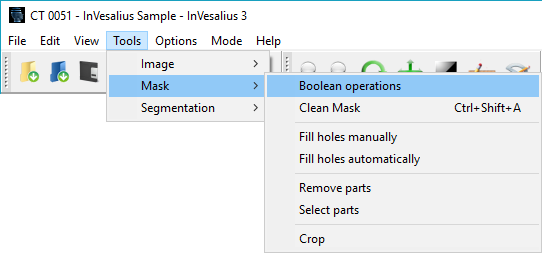
\includegraphics[scale=0.5]{mask_operation_boolean_menu_en.png}
\caption{Menu to open boolean operations tool.}
\label{fig:booleano_menu}
\end{figure}

It's necessary to select the select the first mask, the operation to be performed and the second mask as shown in the figure~\ref{fig:booleano_janela}. Then click on the \textbf{Ok} button.

\begin{figure}[!htb]
\centering
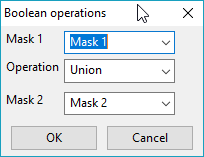
\includegraphics[scale=0.5]{mask_boolean_dialog_en.png}
\caption{Boolean operations tool.}
\label{fig:booleano_janela}
\end{figure}

The figure~\ref{fig:op_boolana} shows some examples of utilization of boolean operations tool.

\begin{figure}[!htb]
  \centering
  \subfloat[Mask A]{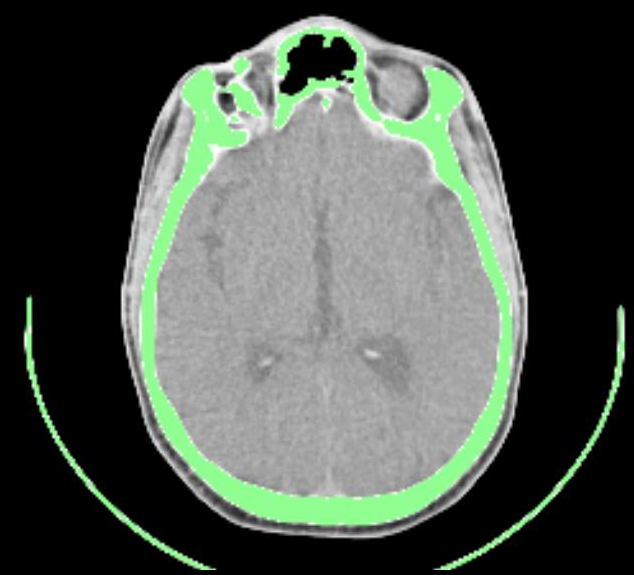
\includegraphics[width=0.332\textwidth]{booleano_m_a.png}}
  \hfill
  \subfloat[Mask B]{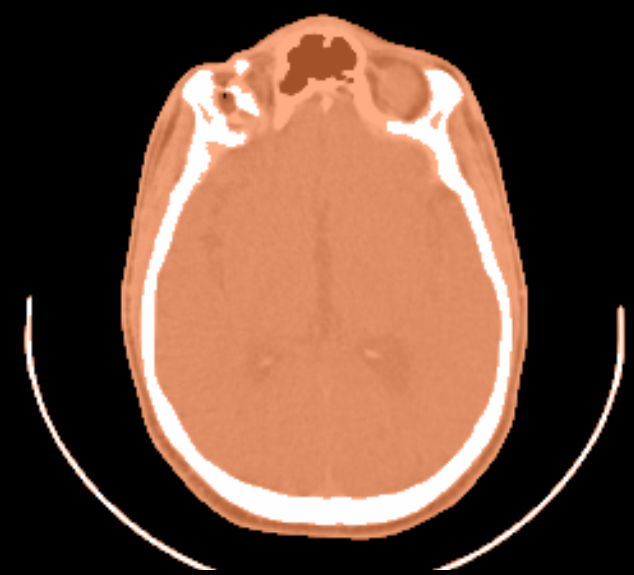
\includegraphics[width=0.332\textwidth]{booleano_m_b.png}}
  \hfill
  \subfloat[Union (A $\cup$ B)]{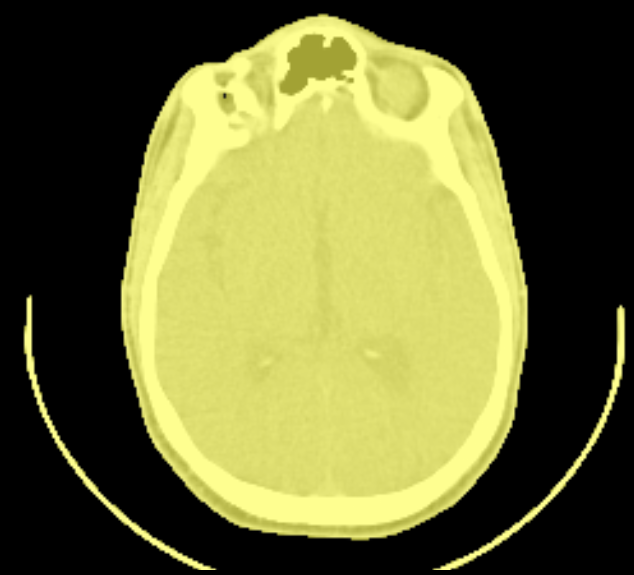
\includegraphics[width=0.332\textwidth]{booleano_uniao.png}}
  \hfill
  \subfloat[Difference (A - B)]{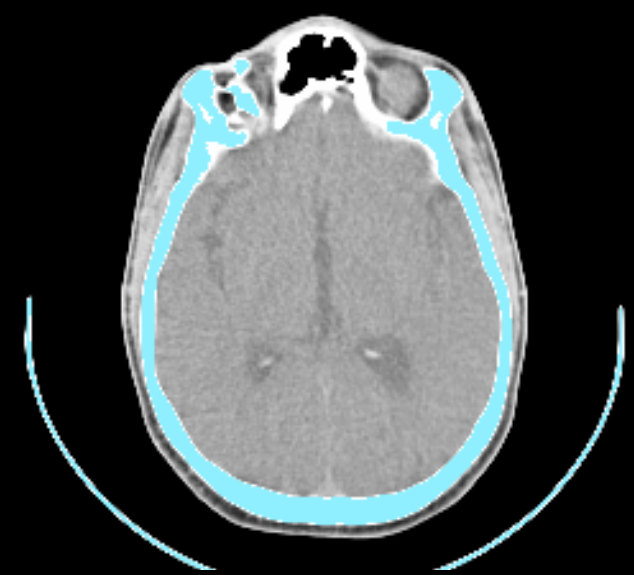
\includegraphics[width=0.332\textwidth]{booleano_dif.png}}
  \hfill
  \subfloat[Intersection (A $\cap$ B)]{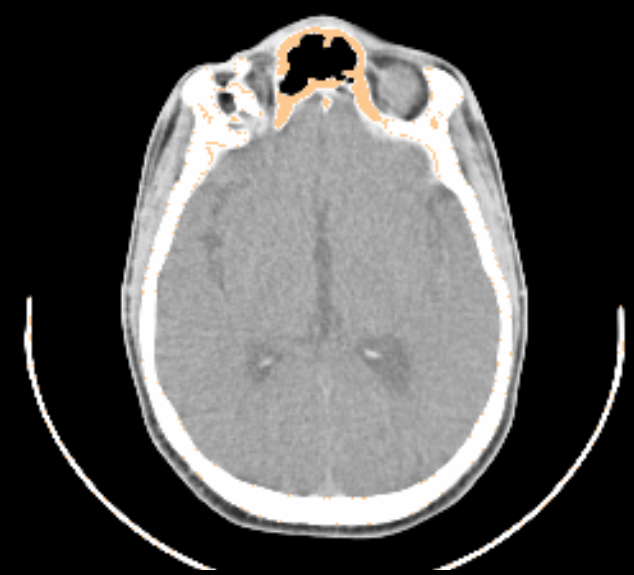
\includegraphics[width=0.332\textwidth]{booleano_interc.png}}
  \hfill
  \subfloat[Exclusive disjunction (A $\oplus$ B)]{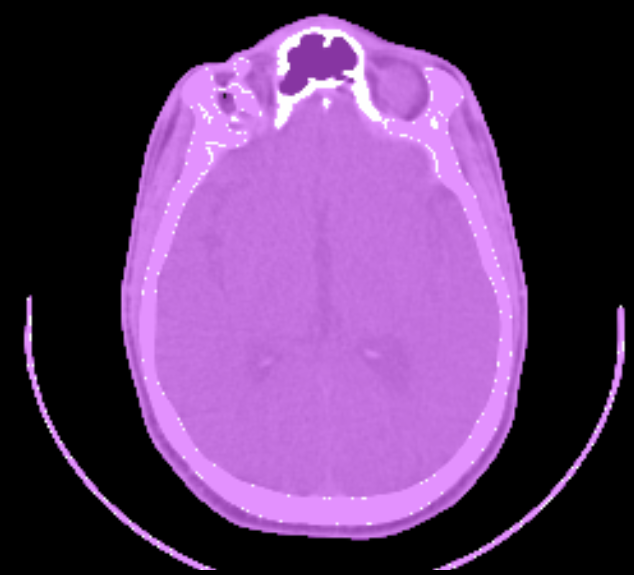
\includegraphics[width=0.332\textwidth]{booleano_disj_exc.png}}
  \caption{example of boolean operations.}
  \label{fig:op_boolana}
\end{figure}

\section{Mask cleaning}
\label{cap:limpeza_mascara}

It's possible to clean a mask (figure~\ref{fig:limpeza_mascara}). This is recommended before starting to insert Watershed markers. This tool is located on menu \textbf{Tools}, \textbf{Mask}, \textbf{Clean mask}. Also, it possible to use keyboard shortcut \textbf{CTRL+SHIFT+A}.

\begin{figure}[!htb]
\centering
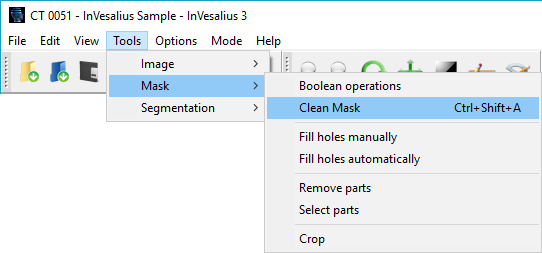
\includegraphics[scale=0.5]{mask_clean_menu_en.png}
\caption{Mask cleaning}
\label{fig:limpeza_mascara}
\end{figure}

\section{Fill holes manually}

Segmentation may leave some unwanted holes. It's recommended to fill them because the surface generated from this mask may have some inconsistencies. To do this access the menu \textbf{Tools}, \textbf{Mask}, \textbf{Fill holes manually} (figure~\ref{fig:menu_mask_manual_fill_holes}). A dialog window will be shown (figure~\ref{fig:mask_manual_fill_holes_window}) to configure the parameters.

\begin{figure}[!htb]
\centering
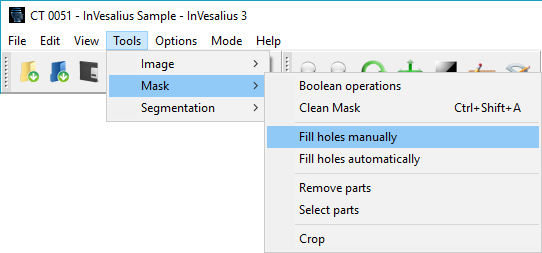
\includegraphics[scale=0.4]{menu_mask_manual_fill_holes_en.png}
\caption{Menu to access the tool to fill holes manually.}
\label{fig:menu_mask_manual_fill_holes}
\end{figure}

\begin{figure}[!htb]
\centering
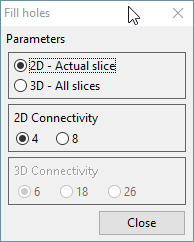
\includegraphics[scale=0.7]{mask_manual_fill_holes_window_en.png}
\caption{Dialog to configure the parameters of Fill holes manually tool.}
\label{fig:mask_manual_fill_holes_window}
\end{figure}

It's possible to fill hole on a mask slice (\textbf{2D - Actual slice}) or on all slices, selecting the option \textbf{3D - All slices}. It's also possible to configure the connectivity used. It may be $4$ or $8$ to 2D and $6$, $18$ and $26$ to 3D.

After configuring the desired parameters click with the \textbf{left-button} of the mouse on holes to fill them.

The figure~\ref{fig:mask_fill_hole}.a shows mask with some holes and other mask with the holes filled (figure~\ref{fig:mask_fill_hole}.b). Click on the \textbf{close} button or close the dialog to deactivate this tool.

\begin{figure}[!htb]
  \centering
  \subfloat[Holes]{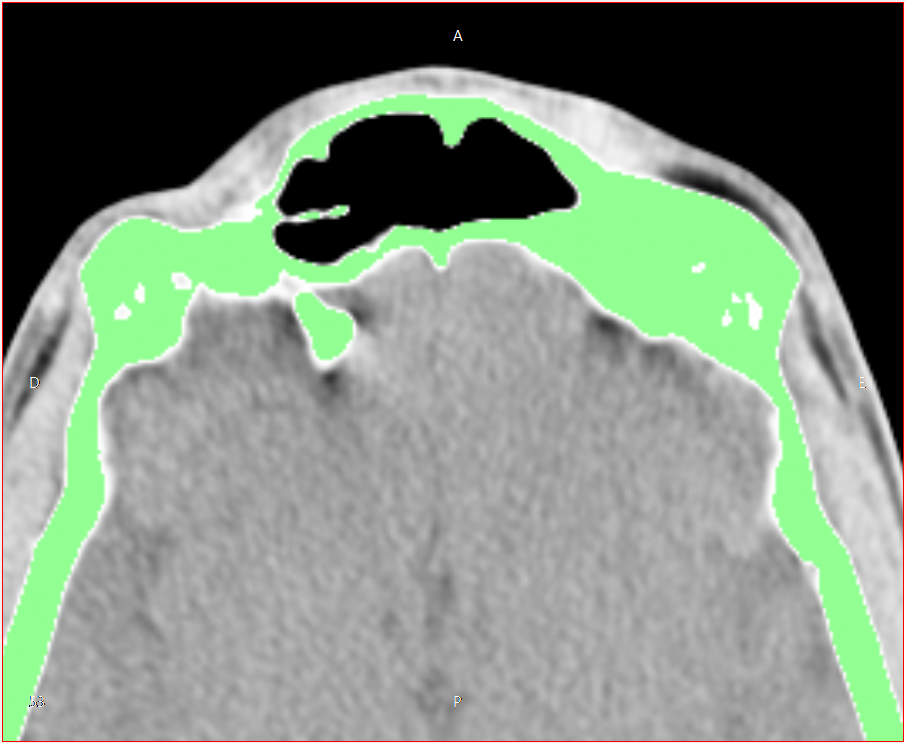
\includegraphics[width=0.4\textwidth]{mask_axial_with_hole.png}}  \qquad
  \subfloat[Holes filled]{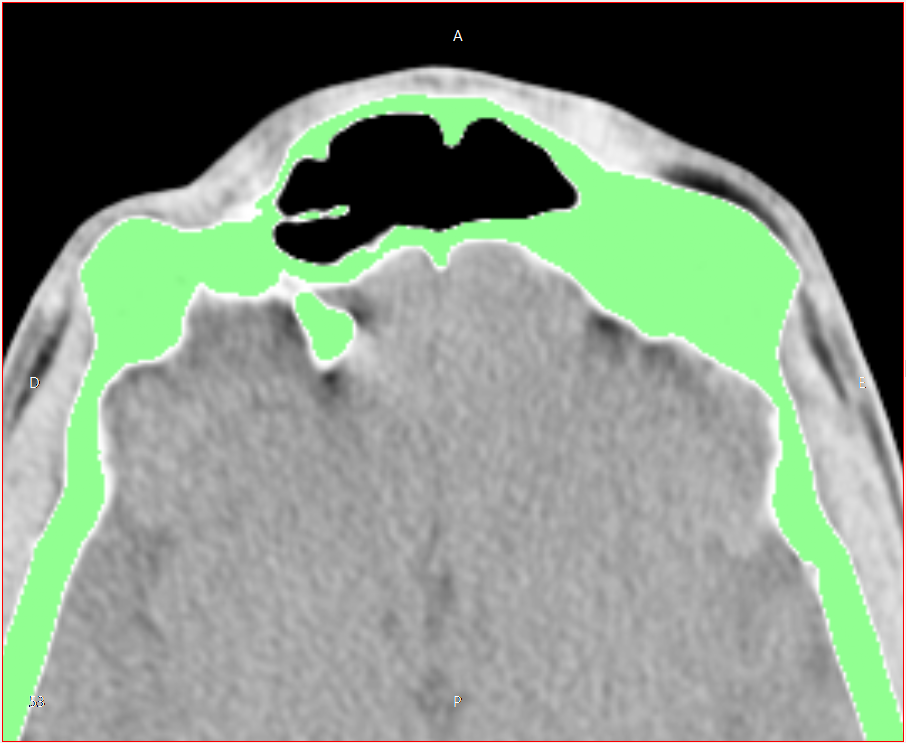
\includegraphics[width=0.4\textwidth]{mask_axial_filled_hole.png}}
  \hfill
  \caption{Example of mask with holes filled.}
  \label{fig:mask_fill_hole}
\end{figure}


\section{Fill holes automatically}

To open this tool go to the menu \textbf{Tools}, \textbf{Mask}, \textbf{Fill holes automatically} (figure~\ref{fig:menu_mask_automatic_fill_holes}). It'll open a dialog to configure the parameters. This tool doesn't require the user to click on holes he desire to fill. This tool will fill the holes based on the \textbf{max hole size parameter} given in number of voxels (figure~\ref{fig:mask_automatic_fill_holes_window}).

\begin{figure}[!htb]
\centering
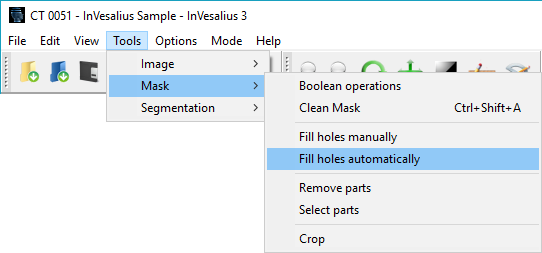
\includegraphics[scale=0.4]{menu_mask_automatic_fill_holes_en.png}
\caption{Menu to open the Fill holes automatically tool.}
\label{fig:menu_mask_automatic_fill_holes}
\end{figure}

\begin{figure}[!htb]
\centering
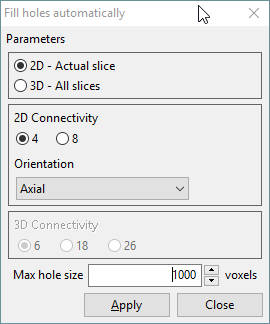
\includegraphics[scale=0.7]{mask_automatic_fill_holes_window_en.png}
\caption{Dialog to configure the parameters used to fill the holes.}
\label{fig:mask_automatic_fill_holes_window}
\end{figure}

It's possible to fill hole on a mask slice (\textbf{2D - Actual slice}) or on all slices, selecting the option \textbf{3D - All slices}. It's also possible to configure the connectivity used. It may be $4$ or $8$ to 2D and $6$, $18$ and $26$ to 3D. In 2D case it's needed to indicate in which orientation window the holes will be filled.

After setting the parameters click in \textbf{Apply} button. If the result is not suitable set other hole size value or try other connectivity. Click on \textbf{Close} button to close this tool.

\section{Remove parts}

After generating a surface is recommended to remove the unwanted disconnected parts from mask. In this way the surface generation will use less RAM and the process will be quicker.  To remove the unwanted parts go the menu  \textbf{Tools}, \textbf{Mask} e \textbf{Remove Parts} (figure~\ref{fig:menu_mask_remove_part}). A dialog will be shown to configure the parameters of selection (figure~\ref{fig:mask_remove_parts_window}).

It's possible to select disconnected part only on a mask slice (\textbf{2D - Actual slice}) or on all slices, selecting the option \textbf{3D - All slices}. It's also possible to configure the connectivity used. It may be $4$ or $8$ to 2D and $6$, $18$ and $26$ to 3D.

\begin{figure}[!htb]
\centering
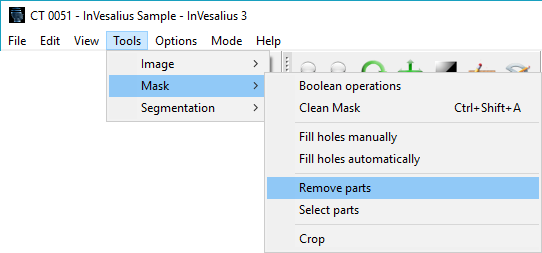
\includegraphics[scale=0.4]{menu_mask_remove_part_en.png}
\caption{Menu to open the Remove parts tool.}
\label{fig:menu_mask_remove_part}
\end{figure}

\begin{figure}[!htb]
\centering
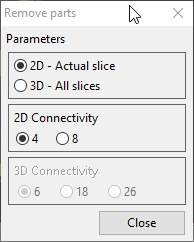
\includegraphics[scale=0.7]{mask_remove_parts_window_en.png}
\caption{Dialog to configure the parameters used in Remove parts.}
\label{fig:mask_remove_parts_window}
\end{figure}

After selecting the desired parameters click with the \textbf{left-button} of the mouse on the region you want to remove. The figure~\ref{fig:mask_removed_part} an example of mask before and after remove a disconnected part. Click on \textbf{Close} button to close this tool.

\begin{figure}[!htb]
  \centering
  \subfloat[Input image]{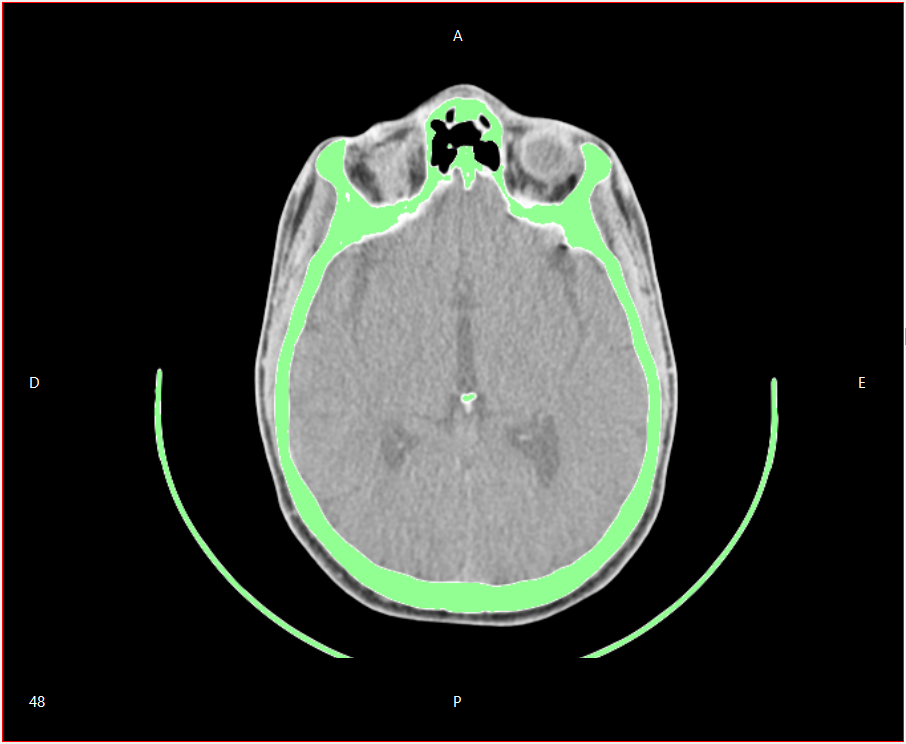
\includegraphics[width=0.45\textwidth]{mask_axial_complete.png}}  \qquad
  \subfloat[Remove the tomograph support]{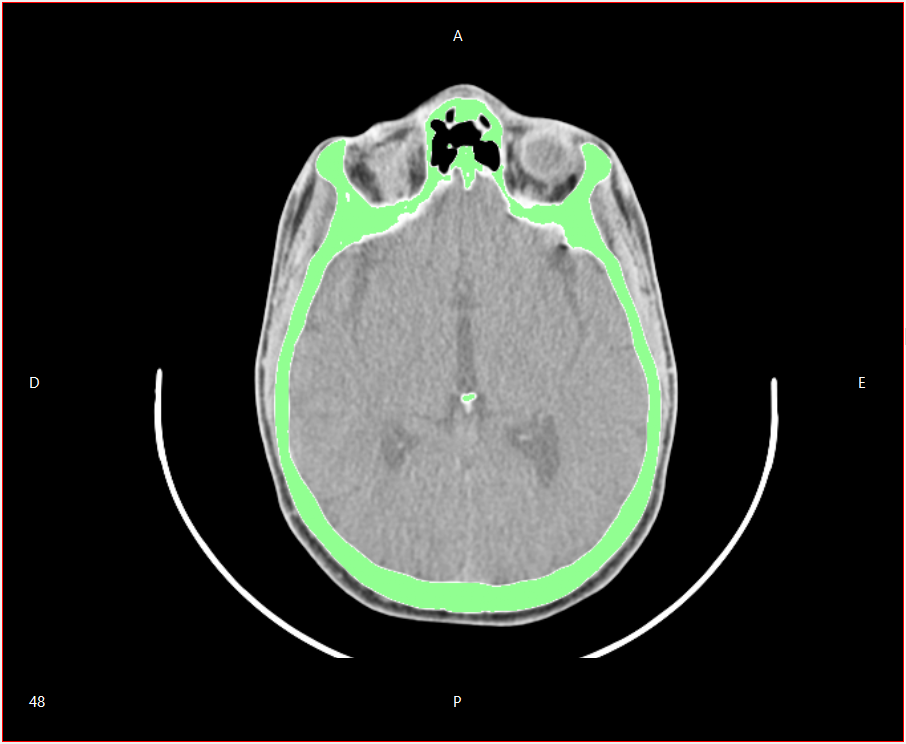
\includegraphics[width=0.45\textwidth]{mask_axial_selected_part.png}}
  \hfill
  \caption{Example of region remove from a mask.}
  \label{fig:mask_removed_part}
\end{figure}

\section{Select parts}

To open Select parts tool go to menu \textbf{Tools}, \textbf{Mask}, \textbf{Select parts} (figure~\ref{fig:menu_mask_select_part}). A dialog will be shown to configure the parameters which are the name of the new mask and the connectivity ($6$, $18$ or $26$).

Click with \textbf{left-button} of the mouse on the wanted pixel of the region you want to select. It's possible to select more than one region. The selected region(s) will be shown with a red mask. After selecting all the wanted regions click on the \textbf{Ok} button to create a new mask with regions selected. The figure~\ref{fig:mask_selected_part}.a shows a region selected in red color. The figure~\ref{fig:mask_selected_part}.b shows the selected region in a new mask.


\begin{figure}[!htb]
\centering
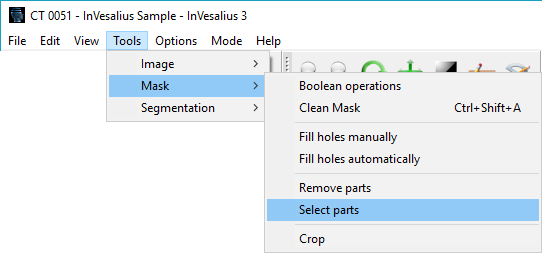
\includegraphics[scale=0.4]{menu_mask_select_part_en.png}
\caption{Menu to open the Select parts tool.}
\label{fig:menu_mask_select_part}
\end{figure}

\begin{figure}[!htb]
\centering
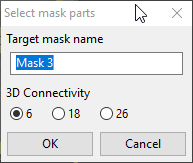
\includegraphics[scale=0.7]{mask_select_part_en.png}
\caption{Dialog to configure the parameters of Select parts tool.}
\label{fig:mask_select_part}
\end{figure}

\begin{figure}[!htb]
  \centering
  \subfloat[Region selected in red]{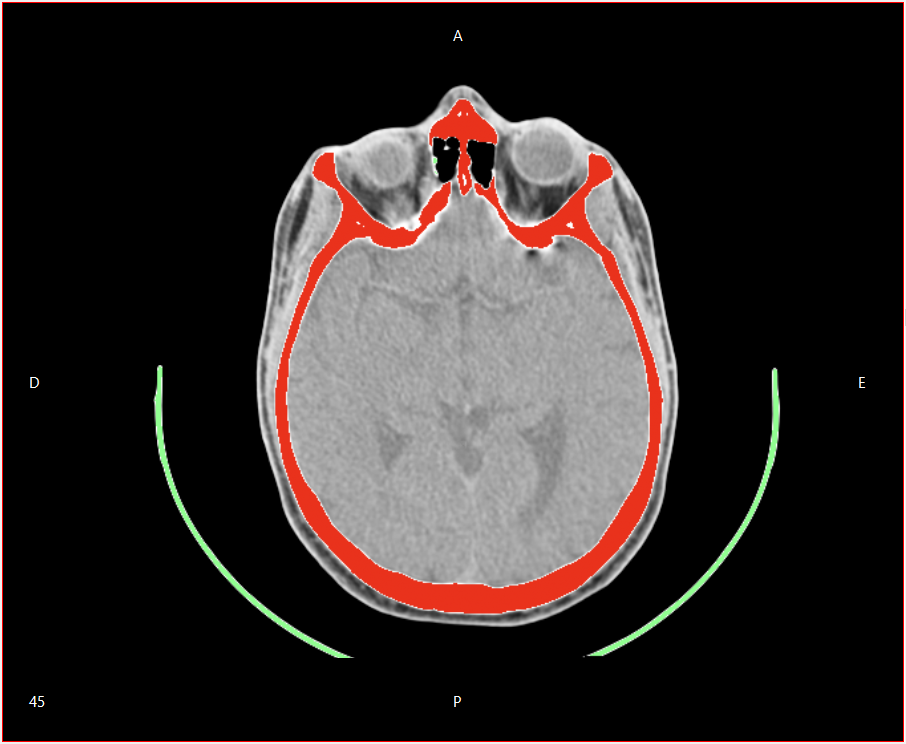
\includegraphics[width=0.45\textwidth]{mask_axial_select_part_pt.png}}  \qquad
  \subfloat[Final image with only the selected region]{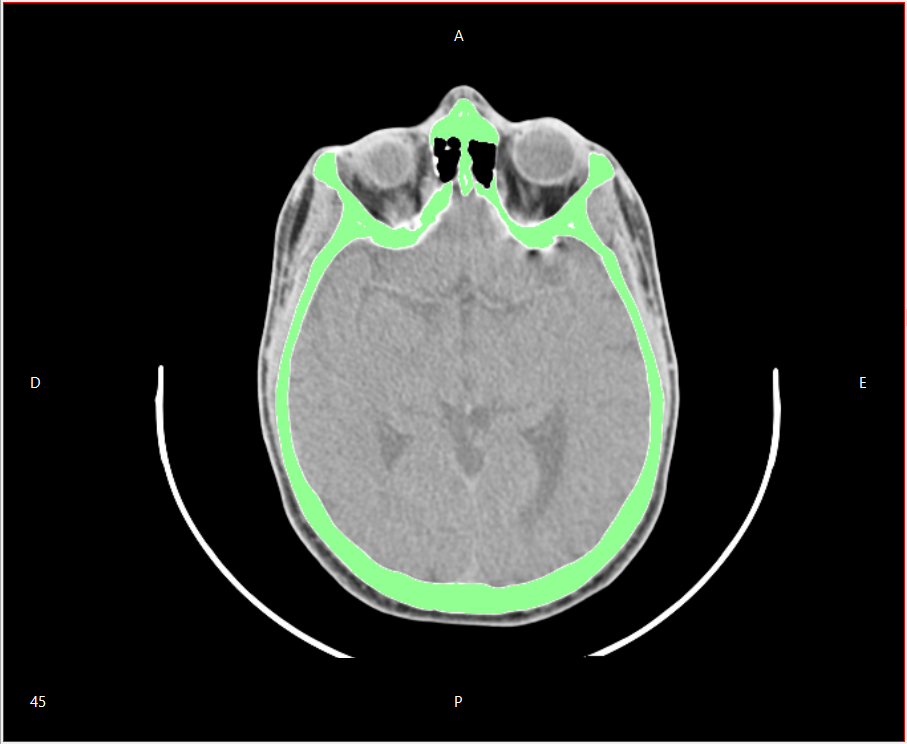
\includegraphics[width=0.45\textwidth]{mask_axial_selected_part_pt.png}}
  \hfill
  \caption{Example of mask region selection.}
  \label{fig:mask_selected_part}
\end{figure}

\section{Crop}

It's possible to cut part of a mask in order to select an region of interest. This may reduce the amount of information to processed when generating a surface. To open this tool go to the menu \textbf{Tool}, \textbf{Mask}, \textbf{Crop} (figure~\ref{fig:menu_mask_crop}).

\begin{figure}[!htb]
\centering
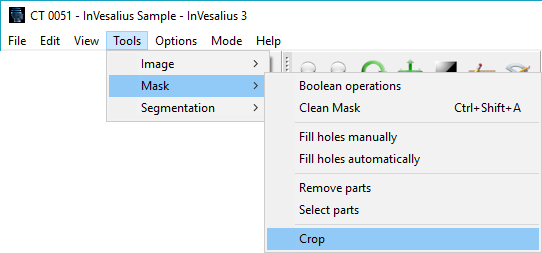
\includegraphics[scale=0.4]{menu_mask_crop_en.png}
\caption{Menu open the Crop tool.}
\label{fig:menu_mask_crop}
\end{figure}

It will be shown a bounding boxes in each orientation window.
